\section{Preliminaries}\label{Sec: examples}
In this section, we introduce the running example, %, a simplification of GENCODE, 
review the notions of \textit{citation views}~\cite{davidson2017model}, {\em view mapping} and {\em validity} of view mappings \cite{wu2018data}, and then show why the \rba\ of \cite{wu2018data} cannot be extended for aggregate queries and views, motivating the need for {\em provenance}.
% discuss why query rewriting using views is not enough for fine-grained citation, and show why the approach in~\cite{wu2018data} works for fine-grained citation in \textit{conjunctive} queries and views but not for \textit{aggregate} queries and views.

\subsection{Running example: GENCODE}\label{subsec:running example}

\begin{figure}[t!]
    \centering
    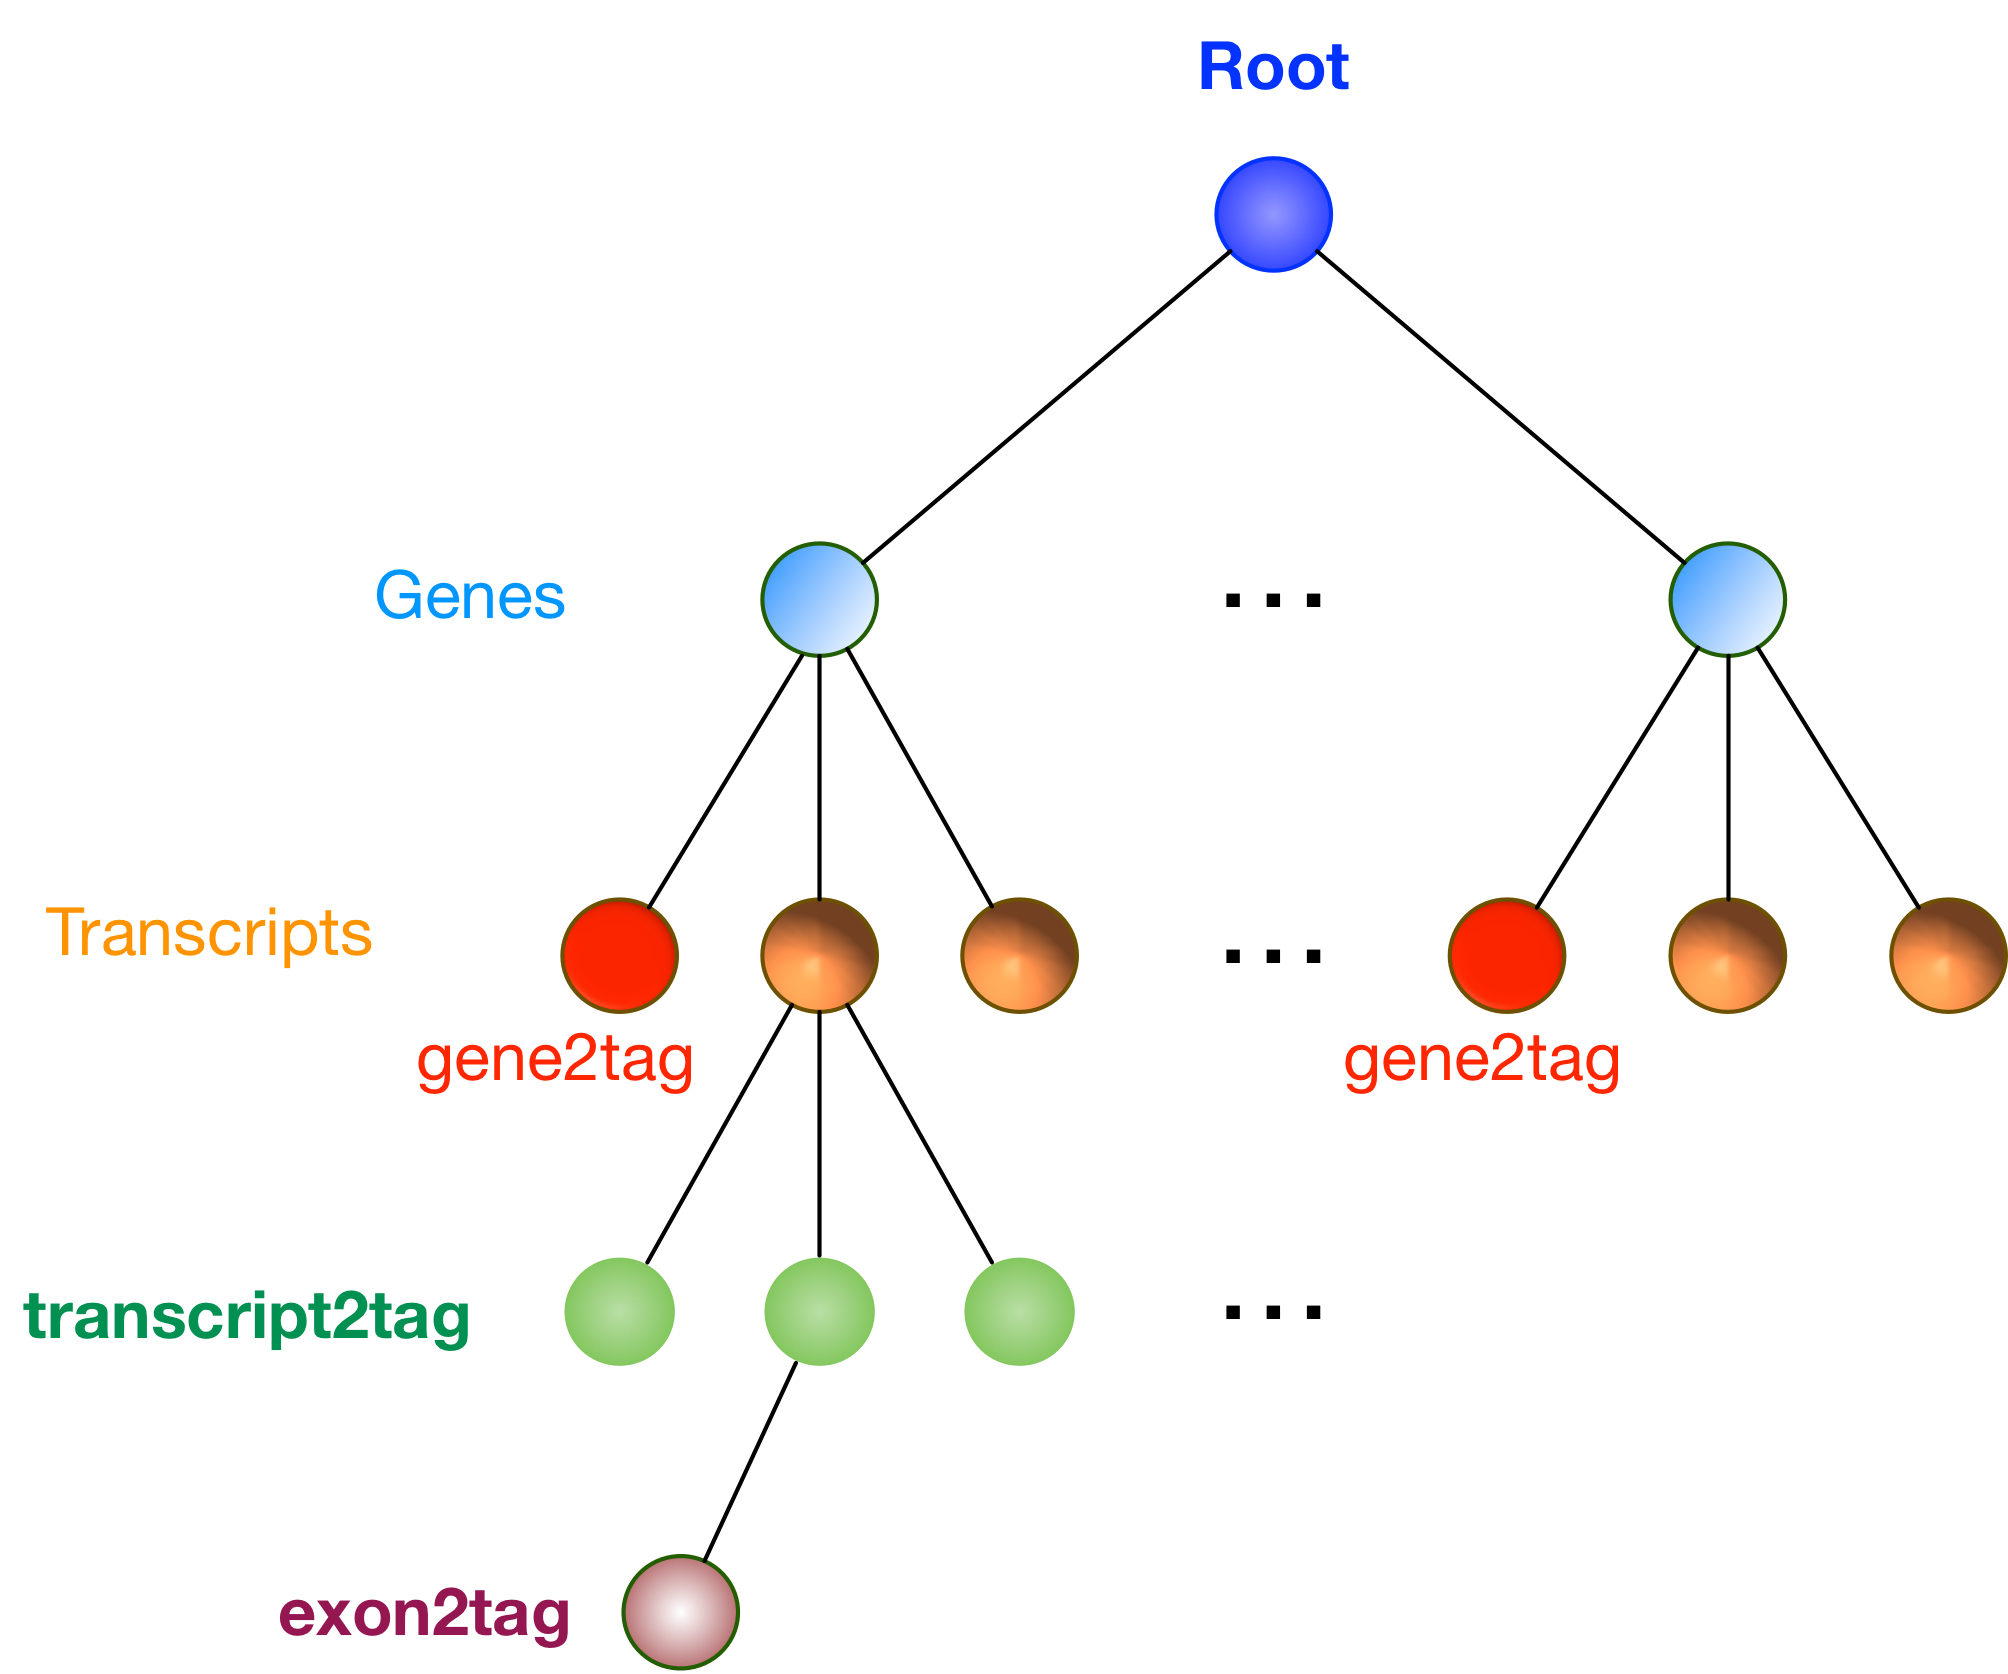
\includegraphics[width=0.4\textwidth,height=0.24\textwidth]{Figures/Gens_Trans_Tree.jpg}
    \caption{Hierarchical structure in GENCODE}
    \small \label{fig:gencode}
\end{figure}


We use a simplified schema from GENCODE as our running example. In this database, information is structured hierarchically (see Figure \ref{fig:gencode}): Each gene is associated with one or more transcripts, and each transcript has one or more exons. Genes, transcripts, and exons may all be annotated with tags, which are created either by human experts or by programs. A simplified schema based on this structure is shown below:

\begin{tabbing}
%\begin{tabular}{l}
Gene(\underline{GID}, Name, Type)\\
Gene2tag(GID, annot) GID references Gene\\
Transcript(\underline{TID}, Name, Type, GID) GID references Gene\\
Transcript2tag(TID, annot) TID references Transcript\\
Exon(\underline{EID}, Level, TID), TID references Transcript\\
Exon2tag(EID, annot), EID references Exon
% \hspace{0.85in} PID references Person\\
% Person(\underline{PID}, PName, Affiliation)\\
% Gene2P(\underline{GID}, \underline{PID}), GID references Gene, PID references Person\\
% Transcript2P(\underline{TID}, \underline{PID}), TID references Transcript, 
% \\PID references Person\\
% Exon2P(\underline{EID}, \underline{PID}), EID references Exon, PID references Person\\
% \hspace{0.85in}  \\
% MetaData(Type, Value)\\
%\end{tabular}
\end{tabbing}
Relations Gene2tag, transcript2tag and exon2tag capture the annotations ({\em annot}). 
% For example, some genes were given annotation ``overlapping locus'', which indicates that ``exon(s) of the locus overlap exon(s) of a readthrough transcript or a transcript belonging to another locus''\footnote{http://vega.archive.ensembl.org/info/about/annotation\_attributes.html}. 
The source of the annotation (e.g. a research group or workflow/program) is also stored in GENCODE and can be used for citations.  For simplicity, we omit these relations.
\eat{
research groups involved in Havana project\footnote{https://www.sanger.ac.uk/science/groups}), which implies citations. Such citation information is also stored in GENECODE and ready for generating formated citations when the corresponding data are cited.}

\textit{Citation views}~\cite{davidson2017model} define views of the database to which citations have been specified.  A citation view consists of 1) a \textit{view query}, defining the subset of the data to which the citation is attached; 2) a \textit{citation query}, which retrieves information required for the citation for the view; and 3) a \textit{citation function}, which formats the information retrieved by the citation query to provide the final citation, e.g. in JSON, BibTex or RIS format. View queries can be considered to be the \textit{frequent queries} over the database; all other queries will be called \textit{general} queries.
\eat{
Since the reasoning involved in generating a citation to a general query involves reasoning over the view queries, we focus on view queries.}

View queries for GENCODE correspond to web-page views  created by the DBAs.  Each of these views could have an associated citation.  For example, the citation query for the web page view of a gene could be used to retrieve the research groups or programs that contributed annotations for the gene; this information, together with the gene name, version of the database, and query used to retrieve the data (e.g. the http address of the web page) could then be formatted by the citation function.
\eat{
For on-line scientific databases like GENCODE, the citation views are defined by DBAs and used to represent the on-line webpages (i.e. cited data) associated with hard-coded citations. For example, for the simplified schema, to mimic those existing citations on line, the {\em view definitions} could be:} 
Below we show several of these views, which are expressed using S-Datalog \cite{consens1990low}, an extended version of Datalog that allows aggregates:
\noindent
\begin{tabbing}
$\lambda G.$\=$V_1(G, N, Ty) $\hspace{4em}\=$:-$\=$ Gene(G, N, Ty)$\\
\> $V_2(G, N, Ty) $\>$:-$\>$ Gene(G, N, Ty)$\\
% \>\>\>$ Exon(E, L, T2), T1=T2$\\
\> $V_3(T1, N1, E, L)$\>$:-$\>$Transcript(T1, N1, Ty1, G1),$\\
% \>\>\>$Gene(G1, N1, Ty1), G1 = G2,$\\
\>\>\>$Exon(E, L, T2), T1 = T2,$\\
\>\>\>$E >= 4$\\
\> $V_4(T1, N1, COUNT(E))$\\
\>\>$:-Transcript(T1, N1, Ty1, G1),$\\
\>\>\>$Exon(E, L, T2), T1 = T2, $\\
\>\>\>$L <= 2$\\
\> $V_5(T1, N1, MAX(L))$\\
\>\>$:-Transcript(T1, N1, Ty1, G1),$\\
\>\>\>$Exon(E, L, T2), T1 = T2$
\end{tabbing}
The first three views are simple conjunctive queries. % and %belong to $\mathcal{CV}$ 
%are simple conjunctive queries.  
$V_1$ is \textit{parameterized} by the gene id $G$, meaning that it defines a family of views, one for each gene. Each view in this family consists of a single tuple.  In this way, each gene may have different citation, giving credit to the person or program who annotated that gene. 
In contrast, $V_2$ and $V_3$ are not parameterized, which indicates that the same citation is shared across all the view tuples. 
\eat{Both $V_1$ and $V_2$ are defined on the Gene relation, and include information about id ($G$), name ($N$) and type ($Ty$).  $V_3$ is a join between Transcript and Exon on Transcript ID ($T1$); the Transcript name ($N1$), Exon ID ($E$) and Exon Level ($L$) are included in the head. 
\scream{Too much detail ... we can assume that people know Datalog?}}
Figure \ref{fig:lambda} shows the effect of the lambda term in $V_1$ versus the unparameterized view $V_2$ on a sample instance of Gene.
% is parameterized by the transcript id $T$,
%and includes the id ($T$), name ($N$) and type ($Ty$) of the transcript, 
% enabling each transcript to have a different citation. 
% The view for each gene and transcript includes information about the 
\begin{figure}[t!]
    \centering
    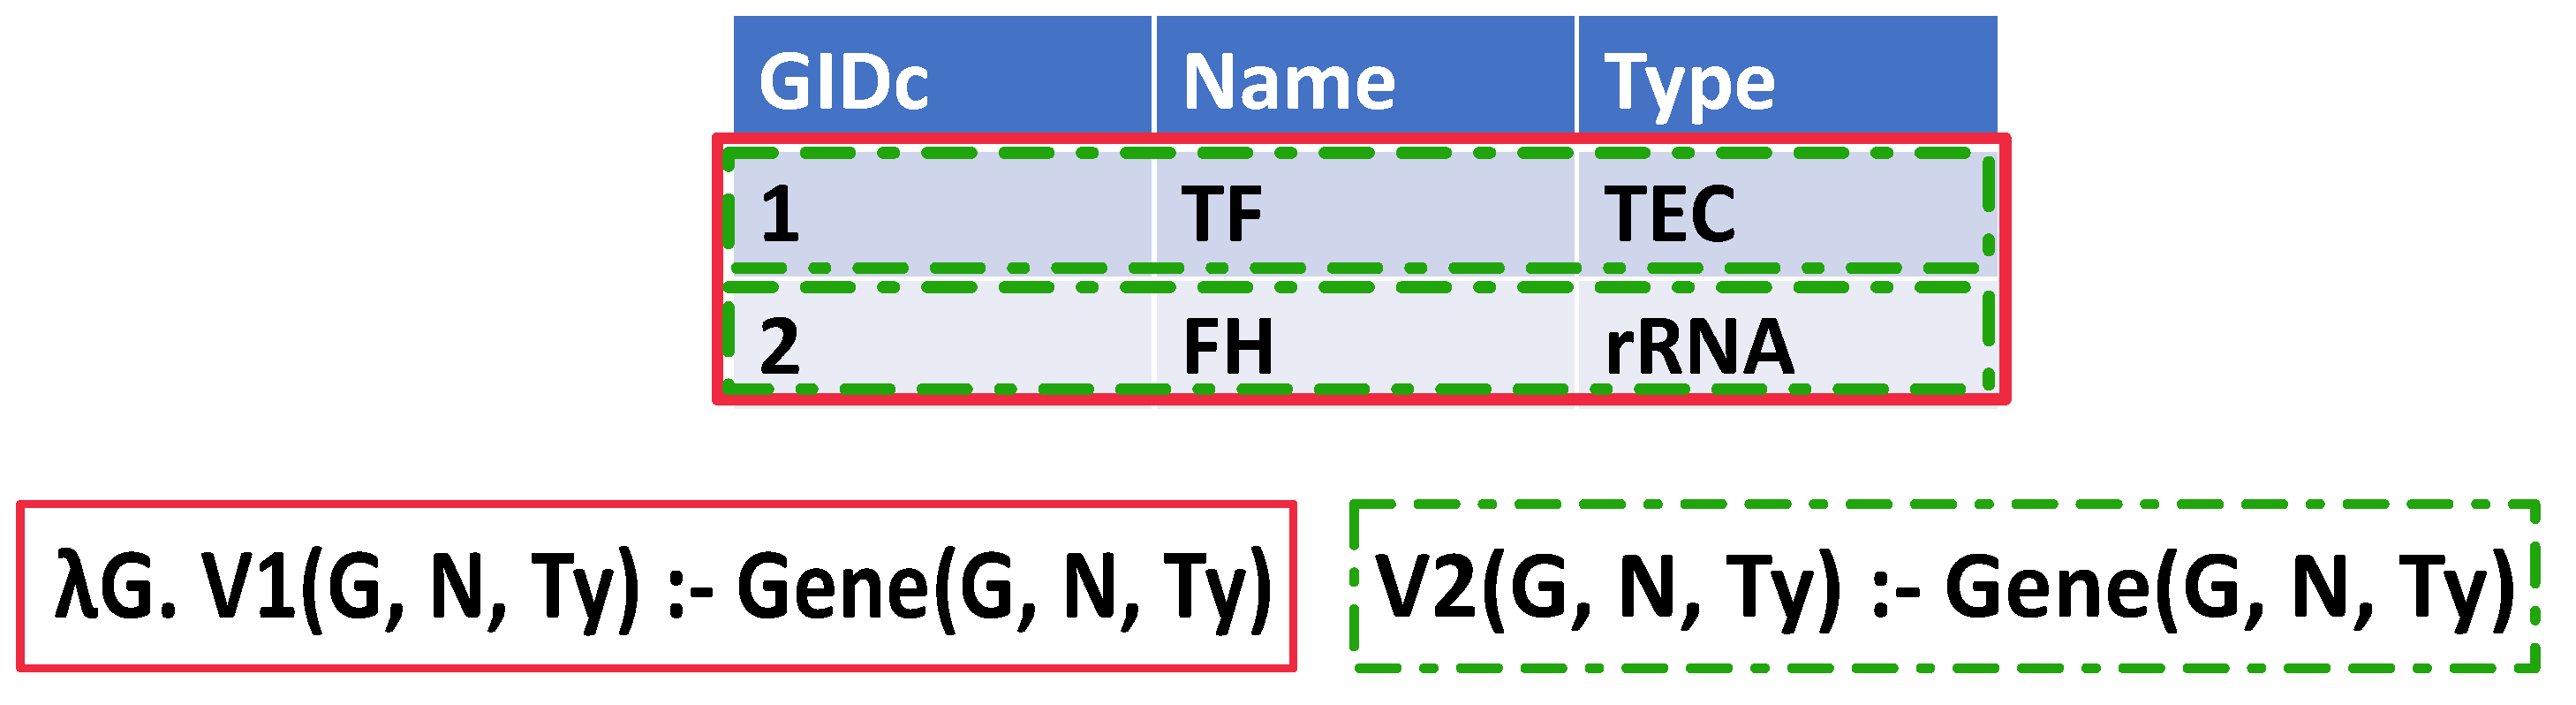
\includegraphics[width=0.45\textwidth,height=0.11\textwidth]{Figures/GIDsExample.pdf}
    \caption{Effect of parameters on views}
    \small \label{fig:lambda}
\end{figure}
The last two views are aggregate views. Their meaning is:  For each binding of variables in the body, group over the variables  in the head (called {\em grouping variables}) and apply the aggregate(s) to each group. Each {aggregate function} along with its arguments is called an {\em aggregate term}, in which the arguments are called {\em aggregate variables}.
Thus $V_4$ could be translated into SQL as:
\begin{tabbing}
SELECT T.TID, T.Name, COUNT(E.EID)\\
FROM Transcript T, Exon E\\
WHERE T.TID=E.TID and E.Level $<=$ 2\\
GROUP BY T.TID, T.Name
\end{tabbing}
$V_4$ counts the number of exons  with level not greater than 2 for each transcript, and includes the transcript name in the result.
$V_5$ returns the maximal level among all exons for each transcript. 

\subsection{Query rewriting:  View mappings}
%\scream{I think we need to cover more concepts here, e.g. the notion of mapping and covering}
Given a (general) query $Q$ and a set of views $\mathcal{V}$, the \rba\ implementation in~\cite{wu2018data} starts by building a set of \textit{view mappings} $\mathcal{M}$ from $\mathcal{V}$ to $Q$. For each query tuple, \rba\ then reasons about the {\em validity} of each view mapping in $\mathcal{M}$ and constructs {\em covering sets}, which are converted to formatted citations later. Each covering set is a \textit{maximal}, \textit{non-redundant} set of {\em valid} view mappings,
% Since there may be many such covering sets, only \textit{maximal}, \textit{non-redundant} covering sets are considered, 
i.e. covering sets for which no other view mappings can be added to \textit{cover} more subgoals and head variables in $Q$, nor can any be removed and still \textit{cover} the same subgoals and head variables in $Q$.

%According to \cite{wu2018data}, a
\eat{here}
A \textit{view mapping} $M$ consists of a {\em relation mapping}, $h$ and {\em variable mapping}, $\phi$ (denoted $M=(h, \phi)$). The former, $h$, maps relational subgoals in a view $V$ to relational subgoals with the same relation names in query $Q$, while the latter variable mapping $\phi$ is an induced mapping by $h$. 
% We say that a head variable of $Q$, $x$ is {\em covered} under $M$ iff there exists a head variable $y$ of $V$ such that $\phi(y) = x$.

Intuitively, for a query tuple $t$, view mapping $M$ is valid iff there exists a view tuple $t'$ in $V$ such that $t'$ is {\em visible} in $t$ under $M$, the reasoning of which depends on examining the lambda variables, the head variables and predicates of views by \rba\ in \cite{wu2018data}. We say that a head variable or a relational subgoal of $Q$ is {\em covered} by $M$ iff it is involved in $M$.

\eat{In the remainder of this paper, we will call the model in \cite{wu2018data} 
the \textit{Rewriting-based Model}.} \eat{maybe we don't need it since we call the approach RBA}

\eat{Need to call this "V\_6" or something... I don't understand the numberings.}

\begin{example}\label{eg: conjunctive_case}
Suppose a conjunctive view and a conjunctive query are defined below:
\begin{tabbing}
$V_{\ref{eg: conjunctive_case}}'(E, T)$\hspace{0.05em}\=$:-$\=$ Exon(E, L, T), E <= 4$\\
%$Q_{\ref{eg: illustrative_eg3}}(Tid, AVG(Level)) $\>$:-$\>$ Exon(Eid, Level, Tid), Tid = 2$
$Q_{\ref{eg: conjunctive_case}}'(Eid, Tid) $\hspace{0.05em}$:- Exon(Eid, Level, Tid)$
\end{tabbing}
There is a view mapping $M_{\ref{eg: conjunctive_case}}' = (h_{\ref{eg: conjunctive_case}}', \phi_{\ref{eg: conjunctive_case}}')$ from $V_{\ref{eg: conjunctive_case}}'$ to $Q_{\ref{eg: conjunctive_case}}'$, in which the relation mapping $h_{\ref{eg: conjunctive_case}}'$ is $\{Exon(E, L, T) \rightarrow Exon$ $(Eid, Level, Tid)\}$ while the variable mapping $\phi_{\ref{eg: conjunctive_case}}'$ is $\{E\rightarrow Eid, L \rightarrow Level, T\rightarrow Tid\}$. $M_{\ref{eg: conjunctive_case}}'$ is only valid for query tuples with $Eid <= 4$ since 1) all the view tuples in $V_{\ref{eg: conjunctive_case}}'$ satisfy $E <= 4$; and 2) no lambda variables in $V_{\ref{eg: conjunctive_case}}'$ and the head variables $E, T$ in $V_{\ref{eg: conjunctive_case}}'$ are mapped to head variables $Eid, Tid$ in $Q_{\ref{eg: conjunctive_case}}'$ respectively, which implies {\em visibility}. For the query tuples for which $M_{\ref{eg: conjunctive_case}}'$ is a valid view mapping, one covering set can be constructed:  \{$M_{\ref{eg: conjunctive_case}}'$\}. After the user selects the query subset or the entire query result,  the \textit{citation queries} associated with $V_{\ref{eg: conjunctive_case}}'$ are executed and the {\em citation function} is applied to construct formatted citations.
\end{example}

% rewriting \textit{each tuple $t$ in the result of} $Q$ in terms of $\mathcal{V}$ (fine-grained citations).  

% Each rewriting involves a subset of the views, whose citations are {\em jointly used} (*) to construct a possible citation for $t$.  Since there may be multiple rewritings for $t$, the citations of each rewriting are {\em alternatively used} (+) to construct the citation for $t$.  Reasoning is done at the level of the schema of views. 



\subsection{The need for provenance}
\label{ssec:need-provenance}
We now show how to reason about the {\em validity} of view mappings for query tuples in the context of aggregate queries and  views via an example, and illustrate why \rba\ fails, motivating the need for {\em provenance}.
% illustrate how aggregate queries can be rewritten in terms of aggregate views, and discuss why the approach is limited in some cases for reasoning about fine-grained citations, necessitating the use of provenance.




\eat{\begin{example}\label{eg: illustrative_eg1}
Suppose we have the following view ($V_{\ref{eg: illustrative_eg1}}$) and query  ($Q_{\ref{eg: illustrative_eg1}}$) defined over relation Transcript:
\eat{\begin{tabbing}
$V_{\ref{eg: illustrative_eg1}}(Ty1, G1, TOP2(T1))$\hspace{0.05em}\=$:-$\=$ Transcript(T1, N1, Ty1, G1)$\\
$Q_{\ref{eg: illustrative_eg1}}(Ty, MAX(T)) $\>$:-$\>$ Transcript(T, N, Ty, G), T <= 3$
\end{tabbing}}
\begin{tabbing}
$V_{\ref{eg: illustrative_eg1}}(T, COUNT(L), SUM(L))$\hspace{0.05em}\=$:-$\=$ Exon(E, L, T)$\\
%$Q_{\ref{eg: illustrative_eg1}}(AVG(Level)) $\>$:-$\>$ Exon(Eid, Level, Tid), Tid <= 3$
$Q_{\ref{eg: illustrative_eg1}}(AVG(Level)) $\hspace{0.05em}$ :- Exon(Eid, Level, Tid), Tid <= 3$
\end{tabbing}


\eat{$V_{\ref{eg: illustrative_eg1}}$ returns the top-2 transcript ids~\footnote{Note that this is not a 1NF result.} for each (gene,type),
whereas $Q_{\ref{eg: illustrative_eg1}}$ returns the largest transcript id for each (type).
It is easy to see that $V_{\ref{eg: illustrative_eg1}}$ can be used to rewrite $Q_{\ref{eg: illustrative_eg1}}$ by further aggregating $V_{\ref{eg: illustrative_eg1}}$ over $Ty$. The reason is as follows: First, there is a {\em view mapping} $M(h, \phi)$ from $V_{\ref{eg: illustrative_eg1}}$ to $Q_{\ref{eg: illustrative_eg1}}$, 
%which is composed of relational subgoal mapping $h$ and variable mapping $\phi$ (See details in \cite{wu2018data}). 
where $h$ maps relational subgoals of $V_{\ref{eg: illustrative_eg1}}$ to relational subgoals of $Q_{\ref{eg: illustrative_eg1}}$ with the same names (i.e. $\{Transcript \rightarrow Transcript\}$) and $\phi$ is an induced variable mapping of $h$ (i.e. $\{T1 \rightarrow T, N1 \rightarrow N, Ty1 \rightarrow Ty, G1 \rightarrow G\}$)~\cite{wu2018data}. Second, under $M$,  $V_{\ref{eg: illustrative_eg1}}$ \textit{does not project out any necessary columns and rows} for computing the query instance; this is done by comparing the head and predicates between the query and view~\cite{srivastava1996answering}. 
Third, there exists a {\em computation rule} from $TOP2$ to $MAX$, which indicates that for the same input, the output of $MAX$ function can be computed using the output of $TOP2$ function~\cite{cohen2006user}. We can therefore say that view mapping $M$ is a valid view mapping at the {\em schema level} for $Q_{\ref{eg: illustrative_eg1}}$~\cite{wu2018data}.}

$V_{\ref{eg: illustrative_eg1}}$ returns the number of exon levels ($COUNT(L)$) and the sum of exon levels ($SUM(L)$) for each Transcript id,
whereas $Q_{\ref{eg: illustrative_eg1}}$ returns the average level for all exons whose corresponding Transcript id is no more than 3.
It is easy to see that $V_{\ref{eg: illustrative_eg1}}$ can be used to rewrite $Q_{\ref{eg: illustrative_eg1}}$ by further aggregating $V_{\ref{eg: illustrative_eg1}}$ over $T$. More formally, this is because:  1) there is a {\em view mapping} $M=(h, \phi)$ from $V_{\ref{eg: illustrative_eg1}}$ to $Q_{\ref{eg: illustrative_eg1}}$, 
%which is composed of relational subgoal mapping $h$ and variable mapping $\phi$ (See details in \cite{wu2018data}). 
where $h$ maps relational subgoals of $V_{\ref{eg: illustrative_eg1}}$ to relational subgoals of $Q_{\ref{eg: illustrative_eg1}}$ with the same names (i.e. $\{Exon \rightarrow Exon\}$) and $\phi$ is an induced variable mapping of $h$ (i.e. $\{E \rightarrow Eid, L \rightarrow Level, T \rightarrow Tid\}$)~\cite{wu2018data}; 2) under $M$,  $V_{\ref{eg: illustrative_eg1}}$ \textit{does not project out any necessary columns and rows} for computing the query instance -- this is checked by comparing the head and predicates between the query and view~\cite{srivastava1996answering}; 
and 3) there exists a {\em computation rule} from $COUNT$ and $SUM$ to $AVG$, which indicates that for the same input, the output of $AVG$ function can be computed using the output of $COUNT$ and $SUM$ function~\cite{cohen2006user}. We can therefore say that view mapping $M$ is a valid view mapping at the {\em schema level} for $Q_{\ref{eg: illustrative_eg1}}$~\cite{wu2018data}.
 
% \scream{Disrupts flow:  (In this case, we say that the aggregate term $AVG(Level)$ in $Q_{\ref{eg: illustrative_eg1}}$ is {\em covered} since the aggregate variable in some aggregate term of $V_{\ref{eg: illustrative_eg1}}$ (say $COUNT(L)$) is mapped to its aggregate variable $Level$ under variable mapping $\phi$) Solved by mentioning it later}

% This is because 1) we can build a view mapping $M$ from $v_{\ref{eg: illustrative_eg1}}$ to $q_{\ref{eg: illustrative_eg1}}$; 2) $v_{\ref{eg: illustrative_eg1}}$ has {\em finer granularity} than $q_{\ref{eg: illustrative_eg1}}$ under the view mapping $M$; 3) we can add a predicate ($T <= 3$) to $v_{\ref{eg: illustrative_eg1}}$ so that $q_{\ref{eg: illustrative_eg1}}$ and $v_{\ref{eg: illustrative_eg1}}$ share the same set of predicates; 4) $v_{\ref{eg: illustrative_eg1}}$ and $q_{\ref{eg: illustrative_eg1}}$ share the same aggregate term, i.e. $MAX(T)$ in their heads (see~\cite{srivastava1996answering} for details).
\end{example}}

% We may also be able relax the last condition (a shared aggregate term) for a view to be usable in a rewriting. % For example:
% \eat{
% It is also possible to relax some conditions in Example \ref{eg: illustrative_eg1} so that the view is still usable to rewrite the query. First, we do a little change to $v_{\ref{eg: illustrative_eg1}}$ and $q_{\ref{eg: illustrative_eg1}}$ such that they do not necessarily share the same aggregate terms in the head under any view mappings. See the following example:}

% \begin{example}\label{eg: illustrative_eg2}
% Suppose we replace $MAX$ in the head of $V_{\ref{eg: illustrative_eg1}}$ with $TOP2$ as shown below, %in $V_{\ref{eg: illustrative_eg2}}$, 
% which computes the largest two values of attribute $T$:

% \begin{tabbing}
% $V_{\ref{eg: illustrative_eg2}}(Ty, G, TOP2(T)) $\hspace{1em}\=$:-$\=$ Transcript(T, N, Ty, G)$\\
% $Q_{\ref{eg: illustrative_eg1}}(Ty, MAX(T)) $\>$:-$\>$ Transcript(T, N, Ty, G), T <= 3$
% \end{tabbing}

% Although $TOP2$ and $MAX$ differ, we can still further aggregate $V_{\ref{eg: illustrative_eg2}}$ over the attribute $Ty$ and take the MAX of the aggregated $TOP2$ values.  This is called a  a {\em computation rule} in~\cite{cohen2006user}.  \eat{That is, we can create a {\em computation rule}~\cite{cohen2006user} $TOP2 \rightarrow MAX$ which, given the same set of values $\bar{X}$, the results of $MAX(\bar{X})$ can be calculated by simply applying a function $f$ over the results of $TOP2(\bar{X})$, i.e. $MAX(TOP2(\bar{X})) = MAX(\bar{X})$. In this case, $v_{\ref{eg: illustrative_eg2}}$ is still a valid candidate to rewrite $q_{\ref{eg: illustrative_eg2}}$.}
% \end{example}

\eat{However, in the context of data citation, we reason about fine-grained citations at the level of a tuple in the output of $Q$,  

Instead of caring about validity of views (or view mappings) in the schema level for any database instance in query rewriting using views problem, we focus on the citations at the tuple level for a given database instance and thus the validity of view mappings for \textit{each query tuple} becomes the priority. Note that it is possible for a view mapping to be valid for a query tuple but not for the entire query result.}
%under every database instance, as shown below:

\begin{example} \label{eg: illustrative_eg3}
%Given  query $Q_{\ref{eg: illustrative_eg3}}$ and $V_{\ref{eg: illustrative_eg3}}$ as follows:
Consider the following query and view:
\begin{tabbing}
$\lambda T. V_{\ref{eg: illustrative_eg3}}'(T, COUNT(L), SUM(L))$\hspace{0.2em}\=$:-$\=$ Exon(E, L, T),$\\
\>\>$COUNT(*) < 3$\\
$Q_{\ref{eg: illustrative_eg3}}'(AVG(Level)) :- Exon(Eid, Level, Tid), Tid <= 4$
\end{tabbing}
% \vspace{-0.5mm}
Note that $V_{\ref{eg: illustrative_eg3}}'$ corresponds to an SQL query with a HAVING clause, since $COUNT(*) < 3$ appears as a subgoal in the body.  $V_{\ref{eg: illustrative_eg3}}'$ is parameterized by $T$, and is associated with a parameterized citation query $CV_{\ref{eg: illustrative_eg3}}'$ which retrieves the citation information for every transcript ID. First, we can derive a view mapping $M_{\ref{eg: illustrative_eg3}}' = (h_{\ref{eg: illustrative_eg3}}', \phi_{\ref{eg: illustrative_eg3}}')$ where $h_{\ref{eg: illustrative_eg3}}' =\{Exon(E, L, T) \rightarrow Exon(Eid, Level, Tid)\}$ and $\phi_{\ref{eg: illustrative_eg3}}' = \{E \rightarrow Eid, L \rightarrow Level, T \rightarrow Tid\}$.
Due to the subgoal $COUNT(*) < 3$, $V_{\ref{eg: illustrative_eg3}}'$ cannot be used to rewrite $Q_{\ref{eg: illustrative_eg3}}'$ since not every tuple in $Q_{\ref{eg: illustrative_eg3}}'(D)$ can be computed using tuples in $V_{\ref{eg: illustrative_eg3}}'(D)$
for \textit{every} database instance $D$.
\eat{, which violates the intuition from ~\cite{srivastava1996answering}, i.e. \textit{the usable views for rewriting a query should not project out any necessary columns and rows for computing the query instance}.}However, \textit{some} query tuples may be still computable from view tuples when a database instance is given.
% by doing further aggregation or applying computation rules.  
Therefore, 
%Since we are interested in individual tuples in {\em fine-grained citation},  
$V_{\ref{eg: illustrative_eg3}}'$ is potentially useful for \textit{fine-grained citations} for \textit{some} tuples in the instance of $Q_{\ref{eg: illustrative_eg3}}'$.
\eat{may be justified, as shown below.
So given a database instance $D$, the usability of $V_{\ref{eg: illustrative_eg3}}$ for generating citations for $Q_{\ref{eg: illustrative_eg3}}$ may be justified, as shown below.}

\eat{Consider the instance of relation Transcript in Table \ref{Table: Sample instance of Transcript}, and the corresponding instances of $V_{\ref{eg: illustrative_eg3}}$ and $Q_{\ref{eg: illustrative_eg1}}$ in Tables \ref{Table: Sample instance of V with provenance} and \ref{Table: Sample instance of Q with provenance}, respectively
(ignore for now the columns containing provenance tokens $a_i$, $b_i$, $c_i$, $d_i$).
Recall that $V_{\ref{eg: illustrative_eg3}}$ groups the first 4 tuples in Transcript by GID and Type, and returns the top-2 TIDs, hence has a set-valued result for TOP2(T).}

To see this, consider the instances of relations Exon, Gene and Transcript in Tables \ref{Instance of Exon}, \ref{Instance of Gene} and \ref{Instance of Transcript} respectively.
%, which are used throughout the rest of the paper. 
Given those instances, the corresponding instances of $V_{\ref{eg: illustrative_eg3}}'$ and $Q_{\ref{eg: illustrative_eg3}}'$ are shown in Tables \ref{Table: Sample instance of V with provenance} and \ref{Table: Sample instance of Q with provenance} (ignore for now the last columns). Note that the citations for each view tuple retrieved by instantiated $CV_{\ref{eg: illustrative_eg3}}'$ are also provided in Table \ref{Table: Sample instance of V with provenance} (see the column with green background).
% Recall that $V_{\ref{eg: illustrative_eg3}}$ groups the first 4 tuples in Exon by Transcript ID, and returns the sum and count of exon levels, hence has a set-valued result for TOP2(T).



\eat{\begin{table}[htp]
\centering
\small
% \caption{Sample instance of relation $Transcript$ with how- and where-provenance}\label{Table: Sample instance of Transcript}
% \begin{tabular}[t]{c|c|c|c|c|c|c|c|c|c|} \hhline{~---------}
% &TID&&Name&&Type&&GID&&\\ \hhline{~---------}
% $t_{1}$&1&$a_1$&TF&$b_1$&TEC&$c_1$&1&$d_1$&$T_1$\\ \hhline{~---------}
% $t_{2}$&2&$a_2$&FH&$b_2$&rRNA&$c_2$&1&$d_2$&$T_2$\\ \hhline{~---------}
% $t_{3}$&3&$a_3$&HP&$b_3$&rRNA&$c_3$&1&$d_3$&$T_3$\\ \hhline{~---------}
% $t_{4}$&4&$a_4$&GK&$b_4$&TEC&$c_4$&2&$d_4$&$T_4$\\ \hhline{~---------}
% $t_{5}$&5&$a_5$&F7&$b_5$&rRNA&$c_5$&1&$d_5$&$T_5$\\ \hhline{~---------}
% \end{tabular}
\caption{Instance of relation $Exon$ with how- and where-provenance}\label{Instance of Exon}
\begin{tabular}[t]{c|c|c|c|c|c|c|c|} \hhline{~-------}
&EID&&Level&&TID&&\\ \hhline{~-------}
$t_{e1}$&1&$e_1$&1&$e_2$&1&$e_3$&$E_1$\\ \hhline{~-------}
$t_{e2}$&2&$e_4$&3&$e_5$&2&$e_6$&$E_2$\\ \hhline{~-------}
$t_{e3}$&3&$e_7$&3&$e_{8}$&2&$e_{9}$&$E_3$\\ \hhline{~-------}
$t_{e4}$&4&$e_{10}$&2&$e_{11}$&4&$e_{12}$&$E_4$\\ \hhline{~-------}
$t_{e5}$&5&$e_{13}$&3&$e_{14}$&5&$e_{15}$&$E_5$\\ \hhline{~-------}
$t_{e6}$&6&$e_{16}$&2&$e_{17}$&5&$e_{18}$&$E_6$\\ \hhline{~-------}
$t_{e7}$&7&$e_{19}$&2&$e_{20}$&5&$e_{21}$&$E_7$\\ \hhline{~-------}
\end{tabular}
\bigskip
\caption{Instance of relation $Gene$}\label{Instance of Gene}
\begin{tabular}[t]{c|c|c|c|c|c|c|c|} \hhline{~-------}
&GID&&Name&&Type&&\\ \hhline{~-------}
$t_{g1}$&1&$g_1$&TF&$g_2$&TEC&$g_3$&$G_1$\\ \hhline{~-------}
$t_{g2}$&2&$g_5$&FH&$g_6$&rRNA&$g_7$&$G_2$\\ \hhline{~-------}
\end{tabular}
\bigskip
\caption{Instance of relation $Transcript$}\label{Instance of Transcript}
\begin{tabular}[t]{c|c|c|c|c|c|c|c|c|c|} \hhline{~---------}
&TID&&Name&&Type&&GID&&\\ \hhline{~---------}
$t_{t1}$&1&$t_1$&MB-203&$t_2$&TEC&$t_3$&1&$t_4$&$T_1$\\ \hhline{~---------}
$t_{t2}$&2&$t_5$&PC-203&$t_6$&rRNA&$t_7$&2&$t_8$&$T_2$\\ \hhline{~---------}
$t_{t3}$&4&$t_9$&HP-218&$t_{10}$&rRNA&$t_{11}$&2&$t_{12}$&$T_3$\\ \hhline{~---------}
$t_{t4}$&5&$t_{13}$&GK-207&$t_{14}$&rRNA&$t_{15}$&2&$t_{16}$&$T_4$\\ \hhline{~---------}
\end{tabular}
\bigskip
\caption{Instance of view $V_{\ref{eg: illustrative_eg3}}$ with provenance}\label{Table: Sample instance of V with provenance}
% \begin{tabular}[t]{c|c|c|c|c|c|c|} \hhline{~------}
% &Ty&&G&&TOP2(T)&\\ \hhline{~------}
% $t_{v_{\ref{eg: illustrative_eg3}}1}$&TEC&$\{c_1\}$&1&$\{d_1\}$&$\{1\}$&$T_1$\\ \hhline{~------}
% $t_{v_{\ref{eg: illustrative_eg3}}2}$&TEC&$\{c_4\}$&2&$\{d_4\}$&$\{4\}$&$T_4$\\ \hhline{~------}
% $t_{v_{\ref{eg: illustrative_eg3}}3}$&rRNA&$\{c_2, c_3\}$&1&$\{d_2, d_3\}$&$\{2,3\}$&$T_2 + T_3$\\ \hhline{~------}
% \end{tabular}
\begin{tabular}[t]{c|c|c|c|c|c|} \hhline{~-----}
&T&&COUNT(L)&SUM(L)&\\ \hhline{~-----}
$t_{v_{\ref{eg: illustrative_eg3}}1}$&1&$\{e_3\}$&1&$1$&$E_1$\\ \hhline{~-----}
$t_{v_{\ref{eg: illustrative_eg3}}2}$&2&$\{e_6, e_9\}$&2&$6$&$E_2 + E_3$\\ \hhline{~-----}
$t_{v_{\ref{eg: illustrative_eg3}}3}$&4&$\{e_{12}\}$&1&$2$&$E_4$\\ \hhline{~-----}
\end{tabular}
\bigskip
\caption{Instance of query $Q_{\ref{eg: illustrative_eg3}}$ with provenance}\label{Table: Sample instance of Q with provenance}
\begin{tabular}[t]{c|c|c|c|c|} \hhline{~----}
&Tid&&AVG(Level)&\\ \hhline{~----}
$t_{q_{\ref{eg: illustrative_eg3}}1}$&2&$\{e_6, e_9\}$&$3$&$E_2 + E_3$\\ \hhline{~----}
$t_{q_{\ref{eg: illustrative_eg3}}2}$&5&$\{e_{15}, e_{18}, e_{21}\}$&$2.33$&$E_5 + E_6 + E_7$\\ \hhline{~----}
\end{tabular}

% \caption{Instance of view $V_{\ref{eg: illustrative_eg3}}$}\label{Table: Sample instance of V}
% \begin{tabular}[t]{c|c|c|c|} \hhline{~---}
% &Type&Gid&TOP2(Tid)\\ \hhline{~---}
% $t_{v_{\ref{eg: illustrative_eg3}}1}$&TEC&1&$\{1\}$\\ \hhline{~---}
% $t_{v_{\ref{eg: illustrative_eg3}}2}$&TEC&2&$\{4\}$\\ \hhline{~---}
% $t_{v_{\ref{eg: illustrative_eg3}}3}$&rRNA&1&$\{2,3\}$\\ \hhline{~---}
% \end{tabular}
% \caption{Instance of query $Q_{\ref{eg: illustrative_eg3}}$}\label{Table: Sample instance of Q}
% \begin{tabular}[t]{c|c|c|} \hhline{~--}
% &Ty&MAX(T)\\ \hhline{~--}
% $t_{q_{\ref{eg: illustrative_eg3}}1}$&TEC&$4$\\ \hhline{~--}
% \end{tabular}
\end{table}}


\eat{In this case, we can further aggregate the view tuples $t_{v_{\ref{eg: illustrative_eg3}}1}$ and $t_{v_{\ref{eg: illustrative_eg3}}2}$ on Type, and apply the computation rule mentioned in Example \ref{eg: illustrative_eg1} over the aggregate term $TOP2(T)$ to compute the query tuple $t_{q_{\ref{eg: illustrative_eg3}}1}$. This strategy works since 1) there is a view mapping $M$ as discussed earlier;
\eat{exists a view mapping $M=(h, \phi)$ where $h=\{Transcript \rightarrow Transcript\}$ and $\phi = \{Tid \rightarrow T, Name \rightarrow N, Type \rightarrow Ty, Gid \rightarrow G\}$}
2) Under the $M$, $V_{\ref{eg: illustrative_eg3}}$ retains all the columns needed by $Q_{\ref{eg: illustrative_eg3}}$; 3) there exist a computation rule from $TOP2$ to $MAX$; 4) The effect of predicates in $V_{\ref{eg: illustrative_eg3}}$ and $Q_{\ref{eg: illustrative_eg3}}$ retain the same set of base relation tuples used to construct the view tuples $\{t_{v_{\ref{eg: illustrative_eg3}}1}, t_{v_{\ref{eg: illustrative_eg3}}2}\}$ and the query tuple $t_{q_{\ref{eg: illustrative_eg3}}1}$, which implies {\em provenance}.}


\begin{table}[htp]
\centering
\small
% \caption{Sample instance of relation $Transcript$ with how- and where-provenance}\label{Table: Sample instance of Transcript}
% \begin{tabular}[t]{c|c|c|c|c|c|c|c|c|c|} \hhline{~---------}
% &TID&&Name&&Type&&GID&&\\ \hhline{~---------}
% $t_{1}$&1&$a_1$&TF&$b_1$&TEC&$c_1$&1&$d_1$&$T_1$\\ \hhline{~---------}
% $t_{2}$&2&$a_2$&FH&$b_2$&rRNA&$c_2$&1&$d_2$&$T_2$\\ \hhline{~---------}
% $t_{3}$&3&$a_3$&HP&$b_3$&rRNA&$c_3$&1&$d_3$&$T_3$\\ \hhline{~---------}
% $t_{4}$&4&$a_4$&GK&$b_4$&TEC&$c_4$&2&$d_4$&$T_4$\\ \hhline{~---------}
% $t_{5}$&5&$a_5$&F7&$b_5$&rRNA&$c_5$&1&$d_5$&$T_5$\\ \hhline{~---------}
% \end{tabular}
\caption{Instance of relation $Exon$ with provenance}\label{Instance of Exon}
\begin{tabular}[t]{c|c|c|c||b|} \hhline{~----}
&EID&Level&TID&prov\\ \hhline{~----}
$t_{e1}$&1&1&1&$e_1$\\ \hhline{~----}
$t_{e2}$&2&3&2&$e_2$\\ \hhline{~----}
$t_{e3}$&3&3&2&$e_3$\\ \hhline{~----}
$t_{e4}$&4&2&4&$e_4$\\ \hhline{~----}
$t_{e5}$&5&3&5&$e_5$\\ \hhline{~----}
$t_{e6}$&6&2&5&$e_6$\\ \hhline{~----}
$t_{e7}$&7&2&5&$e_7$\\ \hhline{~----}
\end{tabular}
\bigskip
\caption{Instance of relation $Gene$ with provenance}\label{Instance of Gene}
\begin{tabular}[t]{c|c|c|c||b|} \hhline{~----}
&GID&Name&Type&prov\\ \hhline{~----}
$t_{g1}$&1&TF&TEC&$g_1$\\ \hhline{~----}
$t_{g2}$&2&FH&rRNA&$g_2$\\ \hhline{~----}
\end{tabular}
\bigskip
\caption{Instance of relation $Transcript$ with provenance}\label{Instance of Transcript}
\begin{tabular}[t]{c|c|c|c|c||b|} \hhline{~-----}
&TID&Name&Type&GID&prov\\ \hhline{~-----}
$t_{t1}$&1&MB-203&TEC&1&$r_1$\\ \hhline{~-----}
$t_{t2}$&2&PC-203&rRNA&2&$r_2$\\ \hhline{~-----}
$t_{t3}$&4&HP-218&rRNA&2&$r_3$\\ \hhline{~-----}
$t_{t4}$&5&GK-207&rRNA&2&$r_4$\\ \hhline{~-----}
\end{tabular}
\bigskip
\caption{Instance of view $V_{\ref{eg: illustrative_eg3}}'$ with provenance and citation}\label{Table: Sample instance of V with provenance}
% \begin{tabular}[t]{c|c|c|c|c|c|c|} \hhline{~------}
% &Ty&&G&&TOP2(T)&\\ \hhline{~------}
% $t_{v_{\ref{eg: illustrative_eg3}}1}$&TEC&$\{c_1\}$&1&$\{d_1\}$&$\{1\}$&$T_1$\\ \hhline{~------}
% $t_{v_{\ref{eg: illustrative_eg3}}2}$&TEC&$\{c_4\}$&2&$\{d_4\}$&$\{4\}$&$T_4$\\ \hhline{~------}
% $t_{v_{\ref{eg: illustrative_eg3}}3}$&rRNA&$\{c_2, c_3\}$&1&$\{d_2, d_3\}$&$\{2,3\}$&$T_2 + T_3$\\ \hhline{~------}
% \end{tabular}
\begin{tabular}[t]{c|c|c|c||a|b|} \hhline{~-----}
&T&COUNT(L)&SUM(L)&citation&prov\\ \hhline{~-----}
$t_{v_{\ref{eg: illustrative_eg3}}'1}$&1&1&$1$&\{Group: [`Lee']\}&$e_1$\\ \hhline{~-----}
$t_{v_{\ref{eg: illustrative_eg3}}'2}$&2&2&$6$&\{Group: [`Joe']\}&$e_2 + e_3$\\ \hhline{~-----}
$t_{v_{\ref{eg: illustrative_eg3}}'3}$&4&1&$2$&\{Group: [`Liu']\}&$e_4$\\ \hhline{~-----}
\end{tabular}
\bigskip
\caption{Instance of query $Q_{\ref{eg: illustrative_eg3}}'$ with provenance}\label{Table: Sample instance of Q with provenance}
\begin{tabular}[t]{c|c||b|} \hhline{~--}
&AVG(Level)&prov\\ \hhline{~--}
$t_{q_{\ref{eg: illustrative_eg3}}'1}$&$2.25$&$e_1 + e_2 + e_3 + e_4$\\ \hhline{~--}
% $t_{q_{\ref{eg: illustrative_eg3}}'2}$&5&$2.33$&$e_5 + e_6 + e_7$\\ \hhline{~---}
\end{tabular}

% \caption{Instance of view $V_{\ref{eg: illustrative_eg3}}$}\label{Table: Sample instance of V}
% \begin{tabular}[t]{c|c|c|c|} \hhline{~---}
% &Type&Gid&TOP2(Tid)\\ \hhline{~---}
% $t_{v_{\ref{eg: illustrative_eg3}}1}$&TEC&1&$\{1\}$\\ \hhline{~---}
% $t_{v_{\ref{eg: illustrative_eg3}}2}$&TEC&2&$\{4\}$\\ \hhline{~---}
% $t_{v_{\ref{eg: illustrative_eg3}}3}$&rRNA&1&$\{2,3\}$\\ \hhline{~---}
% \end{tabular}
% \caption{Instance of query $Q_{\ref{eg: illustrative_eg3}}$}\label{Table: Sample instance of Q}
% \begin{tabular}[t]{c|c|c|} \hhline{~--}
% &Ty&MAX(T)\\ \hhline{~--}
% $t_{q_{\ref{eg: illustrative_eg3}}1}$&TEC&$4$\\ \hhline{~--}
% \end{tabular}
\end{table}


Although $V_{\ref{eg: illustrative_eg3}}'$ and $Q_{\ref{eg: illustrative_eg3}}'$ do not have the same aggregate terms, there exists a \textit{computation rule}~\cite{cohen2006user} from $COUNT$ and $SUM$ to $AVG$:  For the same input, the output of $AVG$ can be computed using the output of $COUNT$ and $SUM$. By applying the computation rule over the aggregate terms $COUNT(L)$ and $SUM(L)$ under view mapping $M_{\ref{eg: illustrative_eg3}}'$, $AVG(Level)$ in query tuple $t_{q_{\ref{eg: illustrative_eg3}}'1}$ is computable. This relies on the fact that: 1) under $M_{\ref{eg: illustrative_eg3}}'$, $V_{\ref{eg: illustrative_eg3}}'$ retains all the columns needed for the aggregation in $Q_{\ref{eg: illustrative_eg3}}'$ (i.e. $Level$); 2) the predicates in $V_{\ref{eg: illustrative_eg3}}'$ and $Q_{\ref{eg: illustrative_eg3}}'$ retain the same set of base relation tuples used to construct the view tuple $t_{v_{\ref{eg: illustrative_eg3}}'1}, t_{v_{\ref{eg: illustrative_eg3}}'2}$ and $t_{v_{\ref{eg: illustrative_eg3}}'3}$ as well as the query tuple $t_{q_{\ref{eg: illustrative_eg3}}'1}$.  Note that this implies {\em provenance}. Intuitively, the aggregate results in $t_{q_{\ref{eg: illustrative_eg3}}'1}$ can be obtained by further aggregation over $t_{v_{\ref{eg: illustrative_eg3}}'1}-t_{v_{\ref{eg: illustrative_eg3}}'3}$ in $V_{\ref{eg: illustrative_eg3}}'(D)$. Meanwhile, citation of $t_{q_{\ref{eg: illustrative_eg3}}'1}$ can be produced by combining the citations of $t_{v_{\ref{eg: illustrative_eg3}}'1}-t_{v_{\ref{eg: illustrative_eg3}}'3}$ , i.e. {\tt \{Group: [`Lee', `Joe', `Liu']\}}.% In contrast, there are no such view tuples for $t_{q_{\ref{eg: illustrative_eg3}}'2}$ since it does not share the same Transcript ID value with any view tuples in $V_{\ref{eg: illustrative_eg3}}'(D)$.

However, it is not trivial to extend \rba\ %in \cite{wu2018data} 
to handle such cases. %aggregate queries and aggregate views. 
The core idea of \rba\ is to determine whether there exists \textit{a} view tuple that can provide a citation to \textit{a} given query tuple (before duplicates are removed), which is achieved by explicitly evaluating the predicates of every view in each individual query tuple. % (See more details in \cite{wu2018data}).
% reason about such connections between \textit{one single} tuple in the view instance and \textit{one single} tuple in the query instance.
% which, from the perspective of provenance, is the same as comparing a how-provenance monomial from the view instance and a how-provenance monomial from the query instance. 
In contrast, every tuple in an aggregate query or aggregate view instance is derived from a \textit{set} of tuples, which complicates the reasoning since we are looking for a group of view tuples that can match {\em exactly} a group of query tuples. 
%The Rewriting-based Model works well for determining the usability of every view tuple in every query tuple, but not for a group of them.
We therefore adopt an alternative model, called the {\em \pbafull} ({\em \pba}).
%Doing such reasoning can be challenging without applying {\em provenance}.
% Doing such reasoning requires {\em provenance}.

\end{example}

